\section{Preliminary Testing on Retrieval}

In this section, we describe the preliminary experiments conducted to evaluate our retrieval system. The primary goal was to compare the baseline Standard RAG approach with our proposed Structured RAG method, which incorporates additional legal structure in the form of citation authority and court hierarchy.

\begin{figure*}[htbp]
  \centering
  \begin{subfigure}[b]{0.52\textwidth}
    \centering
    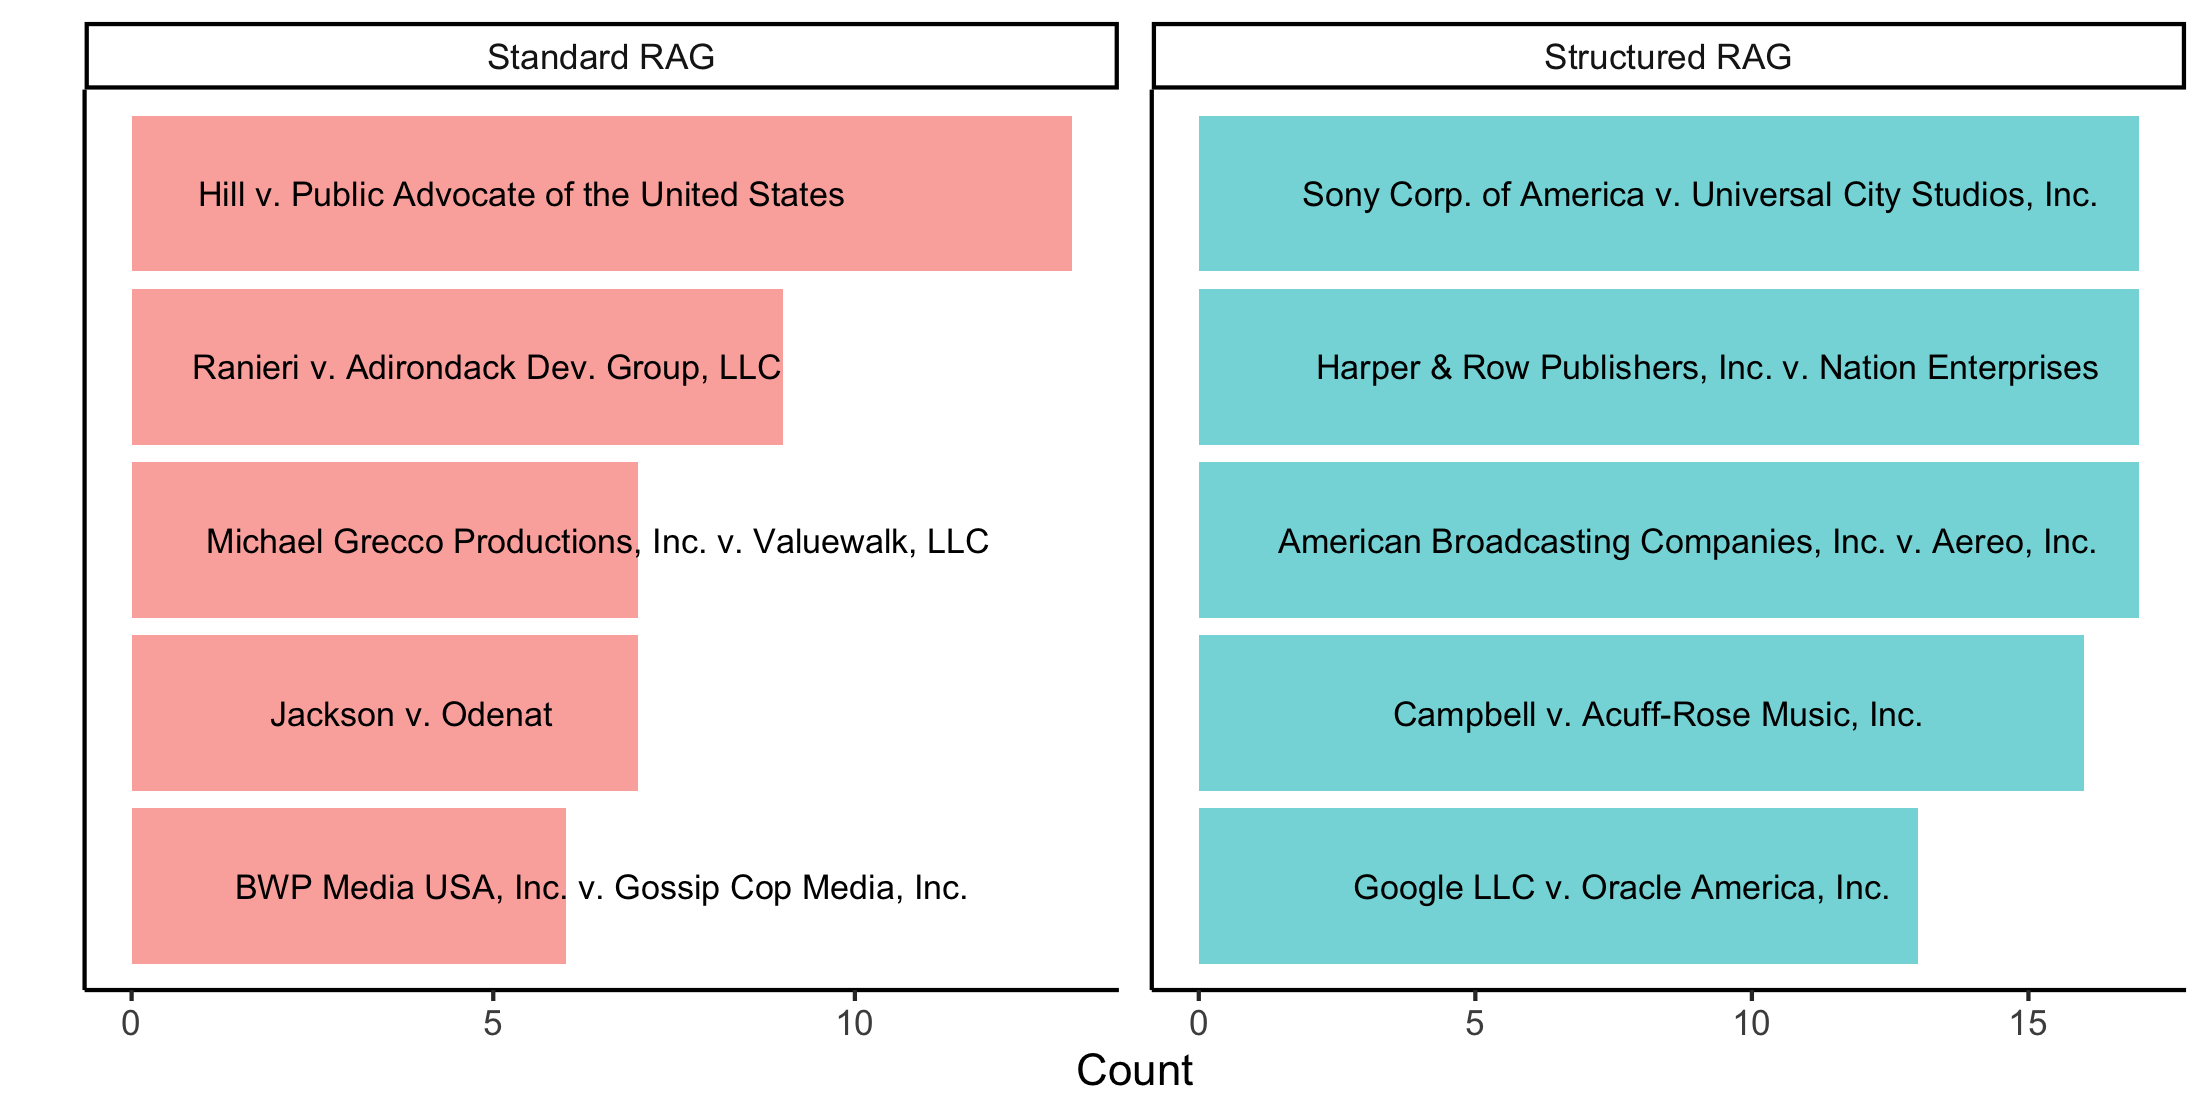
\includegraphics[width=\textwidth]{Top_Cases.png}
    \caption{Most Commonly Retrieved Cases in Each Retrieval Method}
    \label{fig:topcases}
  \end{subfigure}
  \hfill % or \quad or \hspace{<length>}
  \raisebox{3ex}{
  \begin{subfigure}[b]{0.4\textwidth}
    \centering
    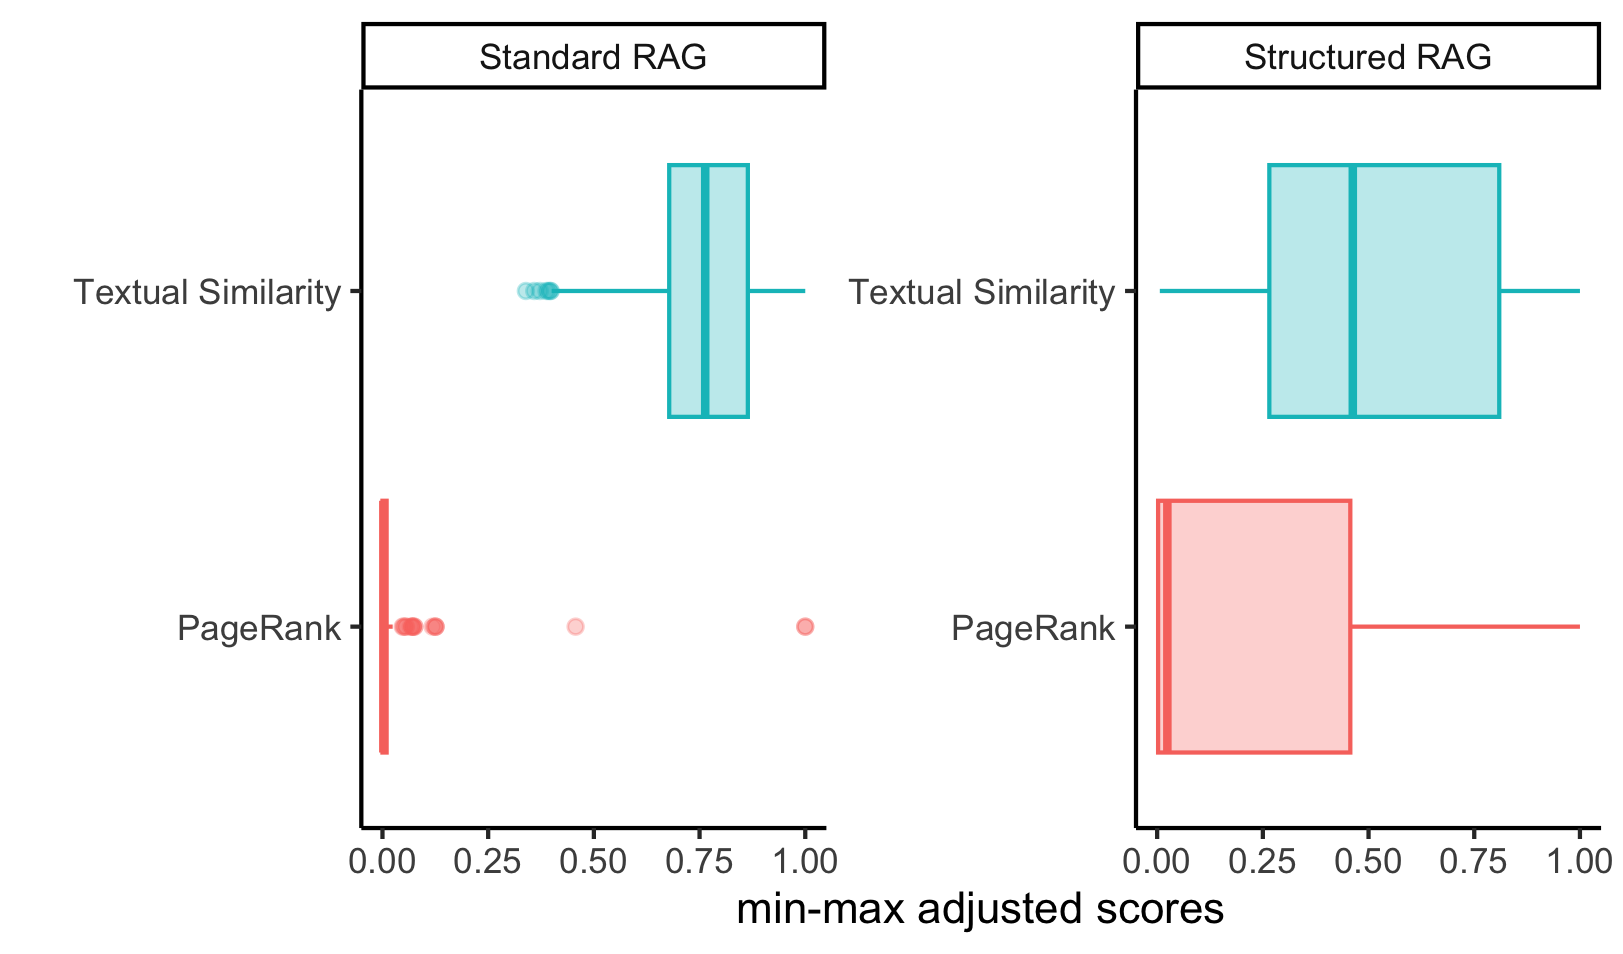
\includegraphics[width=\textwidth]{metric_comparison.png}
    \caption{Boxplot of scores for retrieved cases under Standard RAG and Structured RAG.}
    \label{fig:metric}
  \end{subfigure}
  }
  \caption{Comparison of Retrieval Methods. The Standard RAG achieves higher textual similarity but lacks doctrinal authority as measured by PageRank, and the most common cases retrieved tend to be less authoritative.}
  \label{fig:combined}
\end{figure*}



\begin{table}[ht]
  \centering
  \caption{Comparison of Retrieval Methods with Grouped Metrics. All scores are min-max scaled.}
  \label{tab:grouped_retrieval_comparison}
  \begin{tabular}{l cc | cc}
  \toprule
  \textbf{Retrieval Method} & \multicolumn{2}{c}{\textbf{PageRank}} & \multicolumn{2}{c}{\textbf{Text Similarity}} \\
  \cmidrule(r){2-3} \cmidrule(l){4-5}
                            & \textbf{Mean}    & \textbf{SD}    & \textbf{Mean}      & \textbf{SD}      \\
  \midrule
  Standard RAG    & 0.026 & 0.114 & 0.753 & 0.169 \\
  Structured RAG  & 0.213 & 0.315 & 0.521 & 0.305 \\
  \bottomrule
  \end{tabular}
  \end{table}
  

We used the unresolved copyright complaints from PACER for our preliminary testing and the experiments were run under two configurations:

\begin{itemize}
  \item \textbf{Standard RAG:} The retrieval process relies solely on textual similarity. The hyperparameters are set \(w_{\text{text}}\) = 1 and \(w_{\text{cit}} = w_{\text{court}}= 0\)
  \item \textbf{Structured RAG:} The retrieval incorporates legal structural elements by assigning uniform weights to each component \(w_{\text{text}} = w_{\text{cit}} = w_{\text{court}} = 0.333\).
\end{itemize}
  
We compared the PageRank score and cosine similarity score (reflecting textual similarity) of the retrieved legal opinions. Unsurprisingly, the Standard RAG achieves high textual similarity (Mean = 0.753, SD = 0.169) but retrieves cases with low doctrinal authority as reflected by its low PageRank scores (Mean = 0.026, SD = 0.114). In contrast, the Structured RAG yields higher doctrinal relevance with significantly increased PageRank scores (Mean = 0.213, SD = 0.315), though its textual similarity is somewhat lower (Mean = 0.521, SD = 0.305) - Figure \ref{tab:grouped_retrieval_comparison}. These findings support our hypothesis that adding legal structural data enhances the retrieval of legally significant cases, and could be a way to reduce problems arising from naive retrieval and inapplicable authority \cite{04b_HallucinationFree}.

However, we want to note that this preliminary testing is limited since (1) PageRank is an imperfect estimate of the doctrinal authority as noted in Section \ref{sec: Methods} and (2) the tradeoff between textual similarity and doctrinal relevance might lead to worse Fair Use analysis.
